\documentclass[acmtog]{acmart}
\usepackage{graphicx}
\usepackage{subfigure}
% Title portion
\title{Assignment 3 : Ray-based Rendering and Loop Subdivision} 
\author{Name:\quad Longtian Qiu  \\ student number: \quad 2018533107
	\\email:\quad qiult@shanghaitech.edu.cn }

% Document starts
\begin{document}
\maketitle

\vspace*{2 ex}


\section{Introduction}

In this assignment, a image is generated at ray-based, which means the image is draw one pixel by another.To achieve ray-based rendering, I generate rays from camera and test every rays’ intersection with objects and walls so as to decide the pixel’s color.In the mean time, every object is processed by loop subdivision to make them look more smooth.

\section{Implementation Details}

Inside <camera.hpp> I implement generate camera’s axis and generate ray function which shoot rays from the camera’s position through screen space.
Inside <directLightingintegrator.hpp> I implement radiance function which calculate one pixel’s color according to the pixel’s position in world space and it’s angle with direct light’s position.
In the mean time, a ray is shoot from the pixel position to the direct light’s position to test whether the pixel is blocked by a object which form a shadow.
Inside <refine.hpp> I implement build_data_struct function which convert the data loaded form obj file to two structures, point and face.
(I abandon structure line for i don’t how to use it and feel unnecessary to use it). To be more specific, main information are store inside point structure such as nearby points and related faces.
In loop_subdivision function I firstly iterate all the faces to generate new points and new faces which consist of new and old points, then with the new points , I update the original points’ position.
At last, I iterate all the points to update the their information so as to points data may go into next round of loop_subdivision.The image of the result will be showed in Figure 1 and Figure 2
Inside <triangleMesh.hpp>, I implement raySingleTriangleIntersection function which is the basis for another functions in this file. The function is given a ray and three points’ index,
We need to test whether the face consist of the given three points intersect the ray and store information in the interaction structure.
In rayIntersection function I implement the intersection test with grid, first i try to find the intersection point of the ray and mesh’s bounding box.
Then I find the index position of the grid’s cell covered the intersection point.
Afterwards, I take a “walk” inside cells according to the direction of the ray and record the cells walked. Finally, I check the intersection of the ray and the faces inside recorded cells.
However the effect isn’t acceptable Figure 3.
In subdivision function I manly rearrange the given data to proper data structure fitting loop_subdivision and build_data_struct and after loop subdivision, I convert the data back to the data structure program can render.
In buildUniformGrid function, I first decide the dimension of the gird.then I iterate each cell of the grid to find the faces intersect with cell and record face’s points’ index.
To find the faces intersect with the cell, I choose to shoot two ray inside the cell to check if any faces  intersect with the ray so as to decide whether it’s inside the cell.

\section{Results}

\begin{figure}[h]
\centering
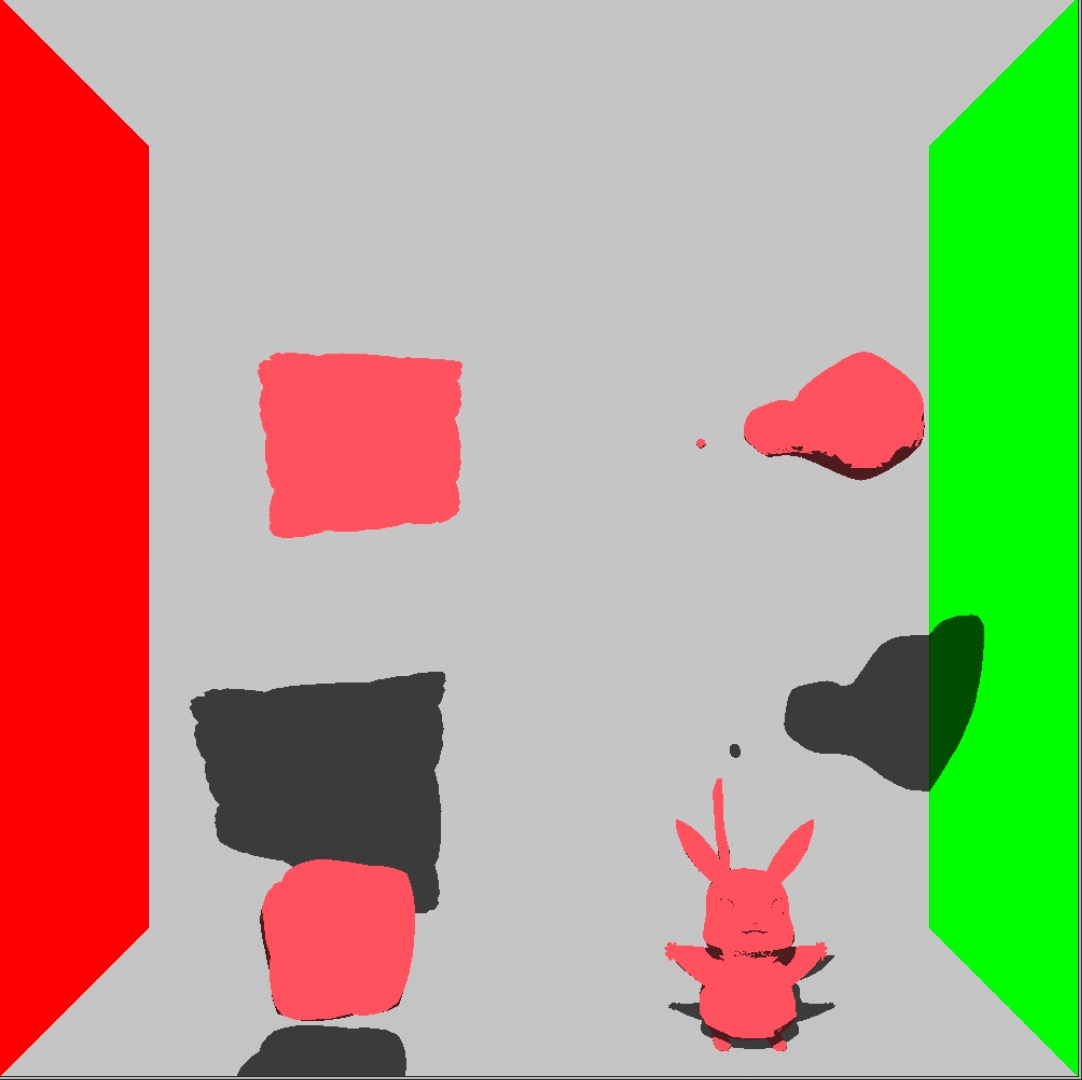
\includegraphics[width=4cm,height=5cm]{complete.jpg}
\caption{With loop subdivision}
\end{figure}

\begin{figure}[h]
	\centering
	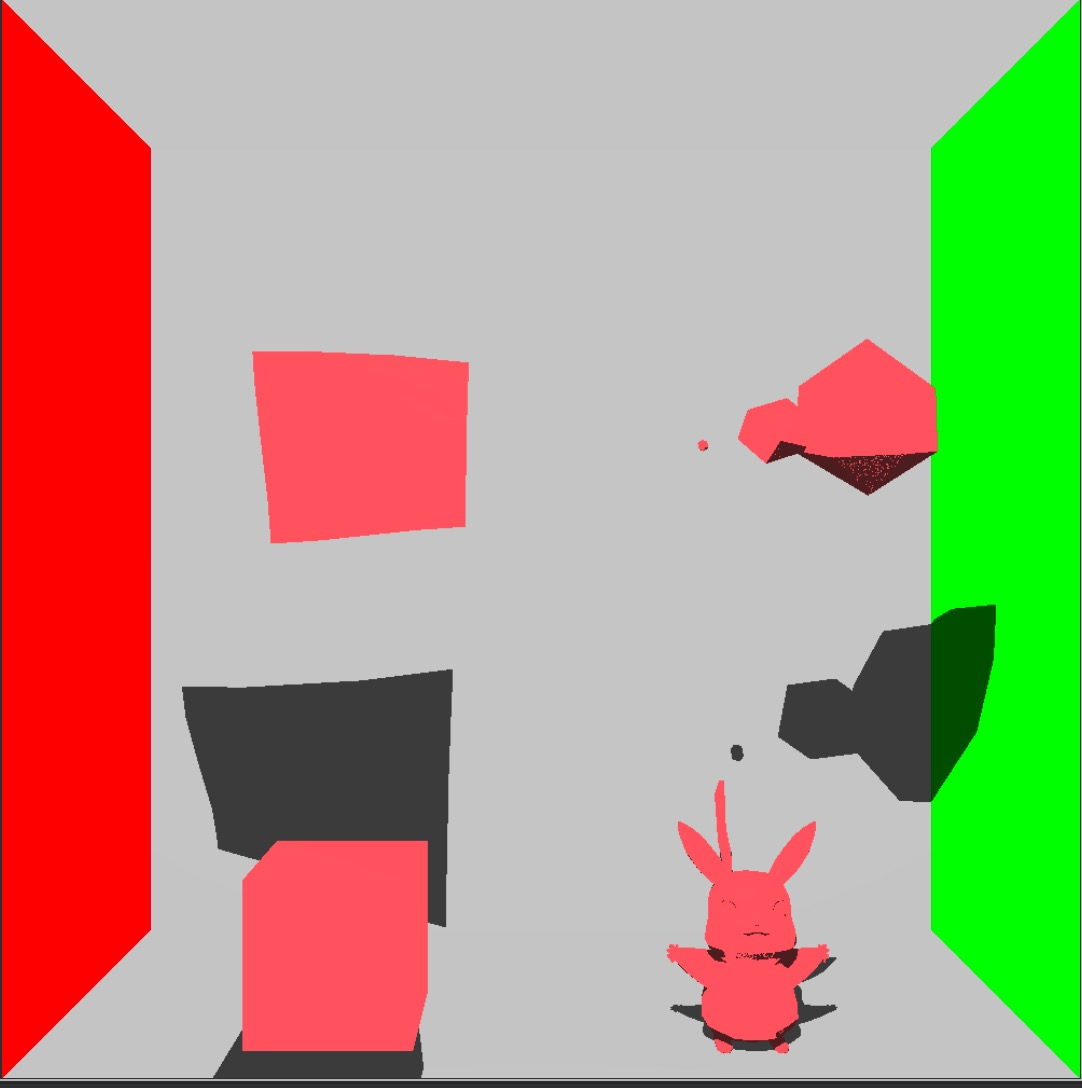
\includegraphics[width=4cm,height=5cm]{no_loop.jpg}
	\caption{Without loop subdivision.}
\end{figure}

\begin{figure}[h]
	\centering
	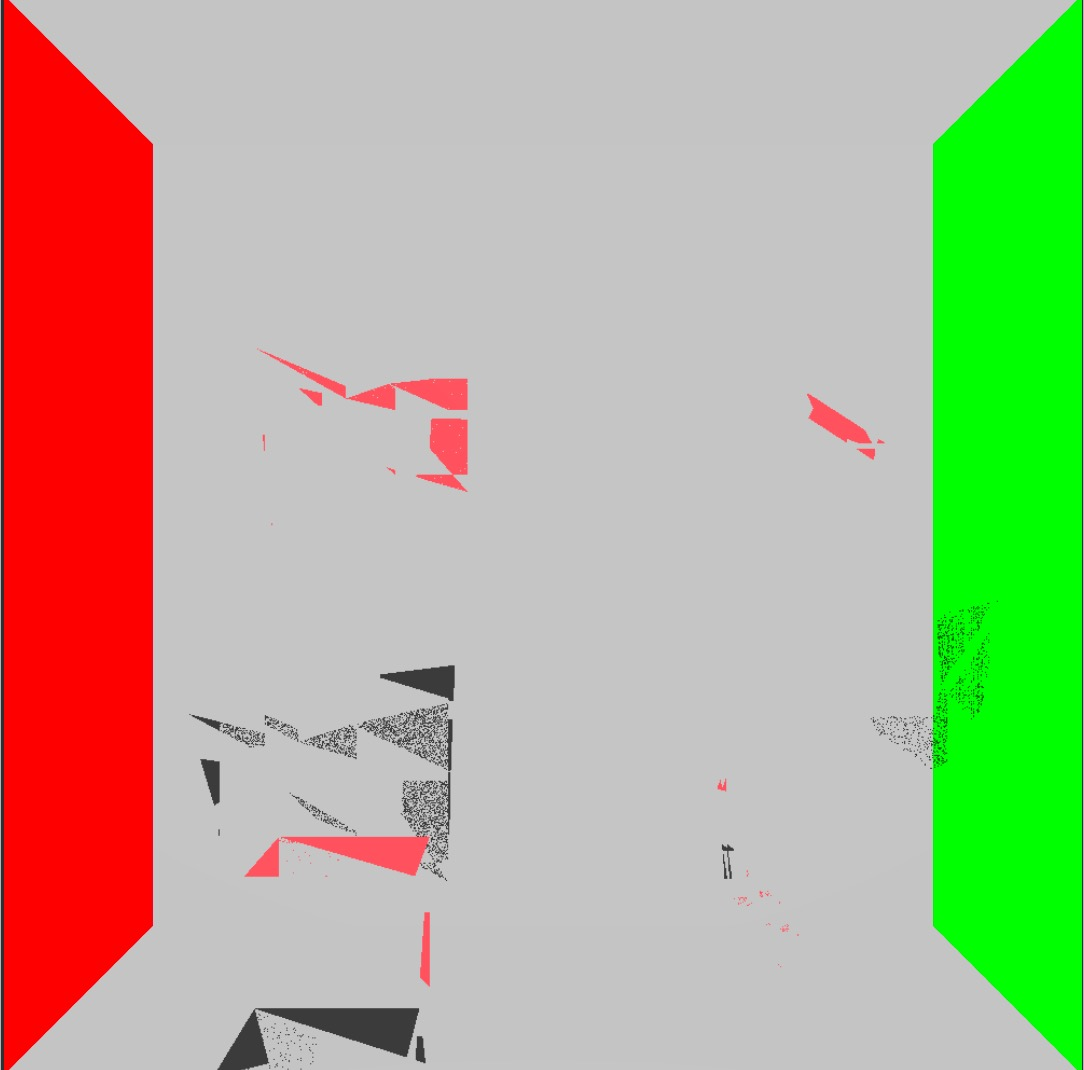
\includegraphics[width=4cm,height=5cm]{grid_fail.jpg}
	\caption{grid failure}
\end{figure}



\end{document}
